\section{Evaluation of Approximation Variance}
\label{sec:estimation-variance}

In this section we will derive a rough quantitaitve estimate of variance of $ \hat f_i$
and then support its credibility by experimental results.

\subsection{Derivation of $Var(\hat f_i)$}
Using the observation that the value $w^*$ chosen by Kmerlight often corresponds
to the analytical $w^*$ and the observation that the value of analytical $w^*$ is a constant
for all $i=1, 2, \dots, m$, we will approximate Kmerlight's variance by a variance
of $t_i^{(w)}$ at the analytically calculated level $w^*$. In this section we will denote
$w^*$ simply as $w$, since we will not use any specific property of $w^*$.


The number of collision-free $k$-mers is equal to the number of collision-free counters
as each collision-free counter stores a single $k$-mer. Thus we will use the symbol
$t_i^{(w)}$ to denote both quantities and it holds that 
$E(t_i^{(w)}) = f_i/2^w \cdot (1 - 1/r)^{F_0/2^w-1}$.

% As the exact probability that from $f_i/2^w$ $k$-mers are exactly $t$
% collision-free can be expressed as 
% ${f_i/2^w \choose t} \cdot P[t ~ k\text{-mers do not collide}] \cdot 
% P[(f_i/2^w - t) ~ k\text{-mers do not collide}]$
% 
% $
% \left(1 - \frac{1}{r}\right)^{F_0/2^w - 1} 
% \left(1 - \frac{1}{r}\right) \left(1 - \frac{1}{r}\right)^{F_0/2^w - 2} 
% \left(1 - \frac{2}{r}\right) \left(1 - \frac{1}{r}\right)^{F_0/2^w - 3}
% {\dots} \left(1 - \frac{t-1}{r}\right) \left(1 - \frac{1}{r}\right)^{F_0/2^w - t}
% $

\paragraph{Sampling View}
In order to approximate the variance of estimator $\hat f_i$ we will consider
$t_i^{(w)}$ to follow a binomial distribution $Bin(f_i, p_s = 1/2^w \cdot (1 - 1/r)^{F_0/2^w-1})$.
This simplification corresponds a simple sampling process in which we sample each a $k$-mer
with probability $p_s$ (sampling probability) and we discard each $k$-mer
with probability $1 - p_s$.

Since a random variable following $Bin(n, p)$ has variance of $np(1-p)$, 
$Var(t_i^{(w)}) = f_i \cdot p_s \cdot (1-p_s)$. The estimate of $f_i$ is obtained
as $t_i / p_s$, so

$$ Var(\hat f_i) = Var \left( \frac{t_i}{p_s} \right) = \frac{1}{p_s^2} \cdot Var(t_i) = \frac{f_i \cdot (1 - p_s)}{p_s} $$

\paragraph{Effect of Medians}
Finally, Kmerlight chooses the estimate $\hat f_i$ as a median of estimates of $t$ 
independent sketches: $\hat f_i = \mathrm{med}(\hat f_i^{(1)}, \dots \hat f_i^{(t)})$.

To incorporate the effect of medians we will use the claim that for a random
variable with a density function $f(x)$ and mean $\bar x$ is its sample median
asymptotically normal:

$$\mathrm{med}(x) ~\dot\sim~ N\left(\bar x, \frac{1}{4nf(\bar x)^2}\right)$$

As the binmoial distribution of $t_i^{(w)}$ is a discrete distribution and does
not have a density function, we will approximate $Bin(f_i, p_s)$ with
$N(\mu = f_i p_s, \sigma^2 = f_i p_s(1-p_s))$. The density function of normal distribution
in the mean is $\frac{1}{\sqrt{2\pi\sigma^2}} e^{-\frac{(\mu - \mu)^2}{2\sigma^2}}$
which is $\frac{1}{\sqrt{2\pi\sigma^2}}$.

Using the two previous approximations, variance of $\hat f_i$ selected as a median of
$t$ instances can be derived as follows:

\begin{equation} \label{eq:variance}
Var(\hat f_i) \approx \left( 4t\frac{1}{2\pi Var(\hat f_i^{(l)})}) \right)^{-1} =
\frac{2\pi}{4t} Var(\hat f_i^{(l)}) = \frac{\pi}{2t} \frac{f_i \cdot (1 - p_s)}{p_s}
\end{equation}


\subsection{Comparison With Experiments}
For low $f_i$, a very small number of $k$-mers hash into collision-free counters at level $w^*$.
Therefore the estimator $\hat f_i$ can reach only a limited set of discrete values (0 if no $k$-mer
survives collisions, 1000 if one $k$-mer is in collision-free counter, 2000 if two $k$-mers survive, \dots),
and the approximation with normal distribution is not precise for $i \in \{ 5, 6, \dots, 14, 15, 40, 41, \dots\}$.

For higher $f_i$, the estimator $\hat f_i$ reaches various values and the approximation with normal distribution
seems reasonable, as it can be seen from figures \ref{img:estimated-pdf} and \ref{img:estimated-cdf}.
These figures show the densities and distribution functions respectively for eight different histogram columns.

We also tried to apply Kolmogorov-Smirnov tests to test the normality of $\hat f_i$. The discrete values of $\hat f_i$
create steps in the cumulative distribution function and therefore these tests reject the normality hypothesis
for the columns with fewer $k$-mers. The hypotheses hold for $f_i > 40000$ ($i \in \{1,2,3,20,21, \dots, 30\}$). 

Nevertheless, in the figures \ref{img:estimated-pdf}, \ref{img:estimated-cdf} it can be
seen that even though the approximation with normal distribution is not precise for the
least frequent abundancies, the $\hat f_i$ can be approximated by gaussian.

\begin{figure}[h]
\centerline{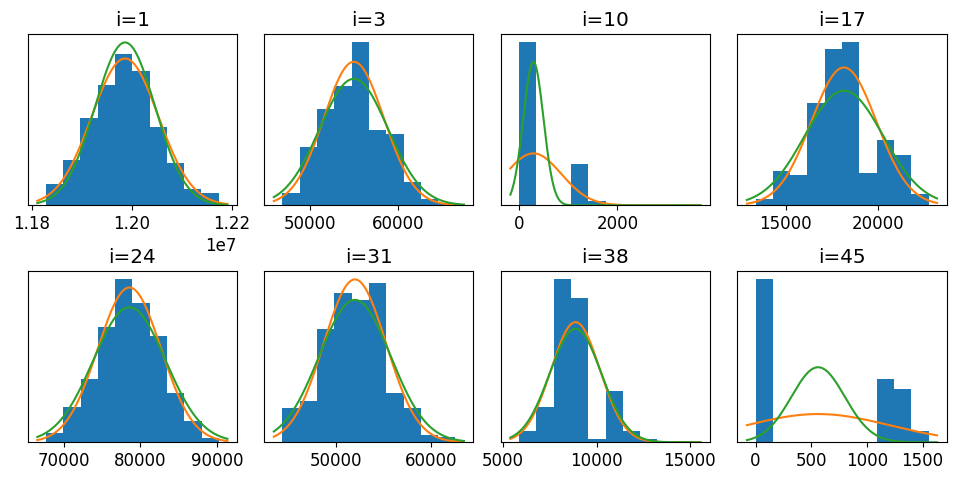
\includegraphics[width=1\textwidth, trim={0cm, 0cm, 0cm, 0cm}, clip]{images/estimated-pdf.png}}
\caption[Density functions of $\hat f_i$]{Probability density (blue histogram), best normal fit (orange line),
theoretical estimate (green) of the distribution of $\hat f_i$. The histogram comes from 300 runs of Kmerlight
with seven instances ($t=7$) and with fixed value of $w^*$. The theoretical prediction uses only the estimated values of 
$f_i$ and $F_0$ to calculate variance that is subsequently used as a parameter for a normal distribution.}
\label{img:estimated-pdf}
\end{figure}

\begin{figure}[h]
\centerline{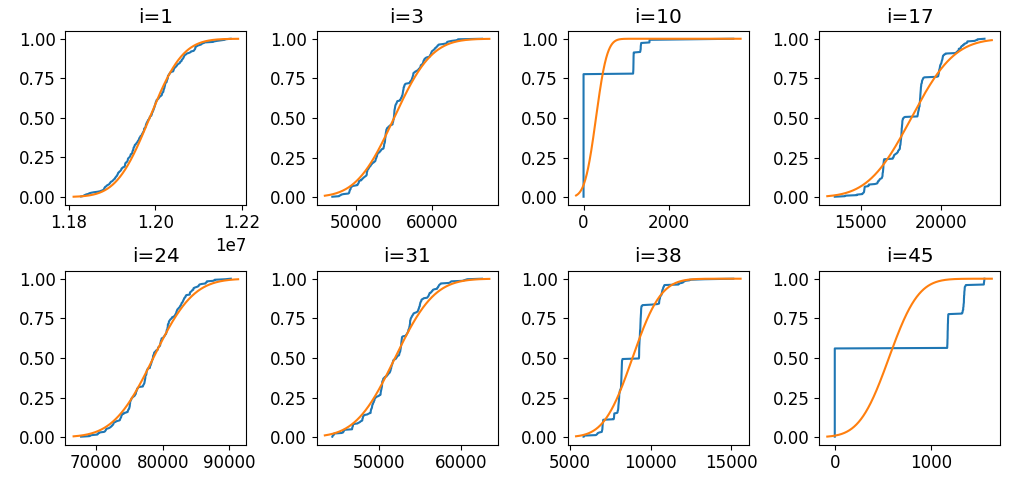
\includegraphics[width=1\textwidth, trim={0cm, 0cm, 0cm, 0cm}, clip]{images/estimated-cdf.png}}
\caption[Distribution functions of $\hat f_i$]{Cumulative distribution funcion (blue), theoretical estimate (orange).}
\label{img:estimated-cdf}
\end{figure}

Finally we present the comparison of the Kmerlight's variance and its theoretical prediction in the
figure \ref{img:std-theory}. Note that our theoretical approximation is based on the fixed value of
level $w^*$ but can also be applied on the original Kmerlight algorithm. 

\begin{figure}[h]
\centerline{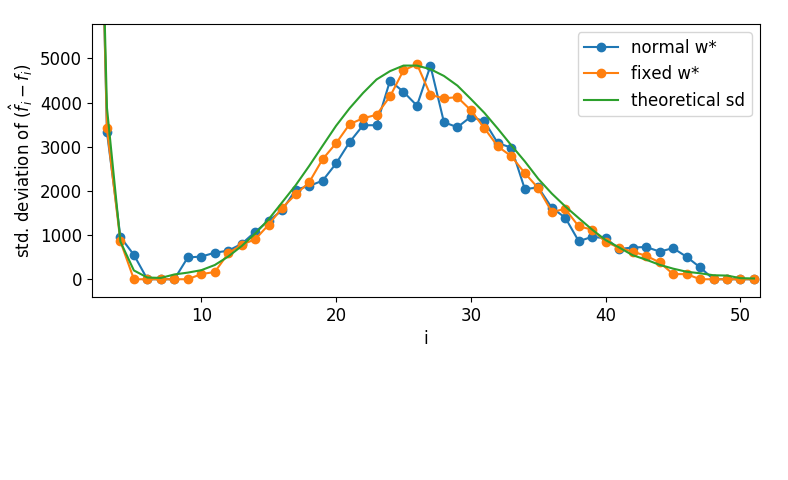
\includegraphics[width=0.9\textwidth, trim={0cm, 3.5cm, 0cm, 0cm}, clip]{images/std_deviations_comparison_theory.png}}
\caption[Experimental and theoretical variance of Kmerlight]{The blue and orange points show standard deviations of $\hat f_i$
computed by original and improved Kmerlight respectively as in the figure \ref{img:std-new-algorithm}. The green line 
represents the approximation of variance calculated with \ref{eq:variance}.}
\label{img:std-theory}
\end{figure}
